\startchapter{Generating Candidates based on Realistic Molecular Model} \label{ch:4}
\section{Description}

After experimenting with the simplified molecule, lacking sufficient spectral information is the key cause for the failure of obtaining the correct target composition. First of all, in the simplified molecule, there are only four vibrational modes, the spectral information is limited. Secondly, the similarity among the candidates is high, as all the candidates are coming from one same molecule. Third, only IR spectra is considered. \\

In this chapter, test cases are conducted using realistic molecules. In addition to IR, both Raman and SFG spectra are calculated for these molecules, which makes the study one step closer to the overall goal and scope. The realistic molecule focused on this chapter is Methionine amino acid. \\

Same as the simplified molecule, in order to limit the possible candidate space of Methionine, $twist$ and $azimuthal$ angular distributions are assumed to be isotropic, which are integrated. Only $\theta$ in Euler angles is considered in Methionine's surface orientation distribution function. In Chapter \ref{ch:2} section Generating model spectra, how a molecule's IR, Raman and SFG spectra are generated have been explained. Two unique IR spectra can be obtained from $x$, and $z$ polarizations. Four unique Raman spectra can be obtained from $xx$, $xy$, $xz$ and $zz$ polarizations. Three unique SFG spectra can be obtained from $xxz$, $xzx$ and $zzz$ polarizations.\\

The goal is to see if those spectral information is sufficient for the LP model to return the correct target composition of the candidates of one type molecule at interfaces. If yes, we need to figure out which spectral information is needed for the LP model. If no, we need to check if the cause of the failure is the same as the simplified molecule. \\

\section{Test Cases}

\begin{table} 
\begin{center}
\begin{tabular}{| l | l | l |  }
\hline
Test Case \# & 1 & 2 \\
\hline
\# Candidates & 4 & 4 \\
\hline
Candidates & [0, 20, 40, 60] & [0, 20, 40, 60] \\
\hline
Target Composition & [0.1, 0.5, 0.4, 0] & [0.1, 0.5, 0.4, 0] \\
\hline
\# Data Points & 200 $x$ & 200 $z$ \\
\hline
%Return Composition & [0.701654, 0, 0, 0.298346] & [0.701654, 0, 0, 0.298346] \\
Return Composition & [0.70, 0, 0, 0.30] & [0.70, 0, 0, 0.30] \\
\hline
\end{tabular} 
\end{center}
\caption{Test Case 1 and 2 setting for methionine candidates} 
\label{tab:4.1}
\end{table}	

\begin{table} 
\begin{center}
\begin{tabular}{| l | l | l | }
\hline
Test Case \# & 3 & 4 \\
\hline
\# Candidates & 4 & 4  \\
\hline
Candidates & [0, 20, 40, 60] & [0, 20, 40, 60]\\
\hline
Target Composition & [0.1, 0.5, 0.4, 0] & [0.1, 0.5, 0.4, 0]\\
\hline
\# Data Points & 200 $x$ + 200 $z$ & 200 $x$ + 200 $xx$\\
\hline
%Return Composition & [0.701654, 0, 0, 0.298346] & [0.1, 0.5, 0.4, 0]\\
Return Composition & [0.70, 0, 0, 0.30] & [0.1, 0.5, 0.4, 0]\\
\hline
\end{tabular} 
\end{center}
\caption{Test Case 3 and 4 setting for methionine candidates} 
\label{tab:case3and4}
\end{table}	

In Table \ref{tab:4.1} and \ref{tab:case3and4}, four test cases are set up with four candidates and same target composition. These four candidates have $\theta$ of the following degree: $0^{\circ}$, $20^{\circ}$, $40^{\circ}$ and $60^{\circ}$. The only difference among these four test cases is the spectroscopy information we select to apply to the LP model, and it is indicated by the Number of Data Points. In Case 1, only $x$-polarized IR spectral information is used. This means that only data points from $x$-polarized IR are selected to apply to the LP model. Same for Case 2, data points are obtained from spectra of IR's $z$-polarized IR. In Test Case 3, the spectral information of $x$ and $z$-polarized IR are combined. At last, in Case 4, spectral information of $x$-polarized IR and $xx$-polarized Raman are combined. Case 4 contains the most abundant information, as its return composition matches to the target one. \\

When merely using IR information, the return composition is the same for Case 1, 2 and 3. Figure \ref{fig:4.1} displays the resulting spectra generated by using the return composition obtained from the first three test cases. The resulting spectra is almost identical to the target ones. It indicates that with only IR spectral information is not sufficient to get the target composition.  However, the spectra built by the return composition matches the target spectra. This means that further information is needed to build the constraints of the LP model. The more constraints are introduced, the more accurate the return composition will be. \\

\begin{figure}[!ht]
\centering
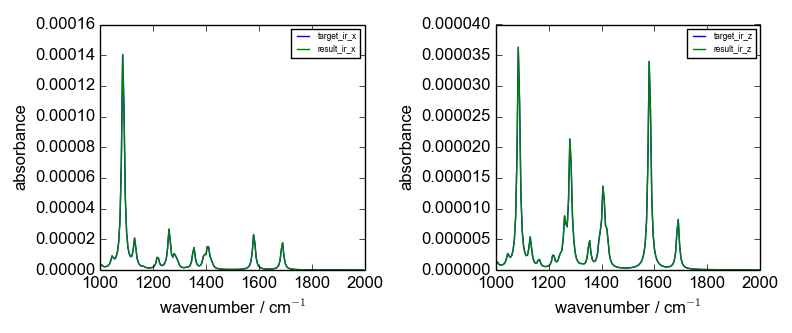
\includegraphics[scale=0.7]{Figures/ir_xz_result_plotting_remove_space.png}
\caption{Compare target IR spectra with the ones generated by the return composition of Case 1, 2 and 3}  \label{fig:4.1}
\end{figure}

In Case 4, combining IR and Raman spectral information is sufficient to obtain the target composition. When the difference in $\theta$ degree for candidates decreases from $20^{\circ}$ to $10^{\circ}$. Checking if Raman and IR together is still sufficient to derive the target composition is desired. Therefore, the following test cases are conducted as shown in Table \ref{tab:4.2}. \\

\begin{table} \tiny 
\resizebox{\textwidth}{!}{
\begin{tabular}{| l | p{3cm} | l | l |}
\hline
\# Candidates & \multicolumn{2}{l|}{4} \\ \hline
Candidates & \multicolumn{2}{l|}{[0, 10, 20, 30]} \\ \hline
Target Composition & \multicolumn{2}{l|}{[0.1, 0.5, 0.4, 0]} \\ \hline
Test Case index & \# Data Points & Result Composition \\ \hline
%5 & 200 $x$ \newline 200 $z$ & [0.752528, 0, 0, 0.247472]  \\ \hline
5 & 200 $x$ \newline 200 $z$ & [0.75, 0, 0, 0.23]  \\ \hline
6 & 200 $x$  \newline 200 $z$ \newline 200 $xx$& [0.1, 0.5, 0.4, 0] \\ \hline
7 & 200 $xx$ \newline 200 $xy$ \newline 200 $xz$& [0.1, 0.5, 0.4, 0] \\ \hline
8 & 200 $xx$ \newline 200 $xy$ \newline 200 $zz$ & [0.1, 0.5, 0.4, 0] \\ \hline
9 & 200 $xx$ \newline 200 $xy$ \newline 200 $xz$ \newline 200 $zz$& [0.1, 0.5, 0.4, 0] \\ \hline
\end{tabular} 
%\end{center}
}
\caption{Test case 5 to 9 setting for methionine candidates}
\label{tab:4.2}
\end{table}	

Case 5 shows that the LP model constructed by merely using IR spectral information is not sufficient to derive the target composition. Case 6 indicates that combining IR and Raman spectral information helps to derive the target composition. What's more, Case 7, 8 and 9, illustrate that Raman spectral information itself is sufficient to obtain the target composition as well. \\

For test case setting in Table \ref{tab:4.1}, \ref{tab:case3and4} and \ref{tab:4.2}, combining IR and Raman spectral information to construct a LP model is sufficient enough to obtain the target composition. In order to study the limitation of the LP model, the complexity of the test case setting needed to be increased. Therefore, another group of test cases are designed as shown in Table \ref{tab:4.3}. There are 5 candidates included in the test cases. Each candidate has $\theta$ with the following degree: $0^{\circ}$, $10^{\circ}$, $20^{\circ}$, $30^{\circ}$ and $40^{\circ}$. The target composition is more complex than previous test cases, each candidate takes 20\% in the mixture. \\

Case 10 applys only IR spectral information to the LP model, and the return composition does not match the target one. Case 11 uses only Raman spectral information, and the return composition does not match to the target neither. Same for Case 12 that uses only SFG spectral information. From Case 13, different kinds of spectral information are combined. In Case 13, IR and Raman spectral information is used to produce the LP model, still the return composition is different from the target one. Case 14 combines Raman and SFG, Case 15 uses IR and SFG, Case 16 cooperates all the three spectral information, however, none of them returns a composition that matches the target one. \\

The results of Case 10 to 16 indicate that even combining all the spectral information of IR, Raman and SFG, it is still not sufficient to attain the target composition for the test cases set up in Table \ref{tab:4.3}. The spectral information we apply to the LP model is showing its limitation in these test cases. In order to confirm the reason causing the LP model to returning the target composition is because of insufficient information, further test cases are conducted in Table \ref{tab:4.4}. \\

\begin{table} \tiny
\begin{center}
\resizebox{\textwidth}{!}{
\begin{tabular}{| l | p{3cm} | l | l |}
\hline
Number of Candidates & \multicolumn{2}{l|}{5} \\ \hline
Candidates & \multicolumn{2}{l|}{[0, 10, 20, 30, 40]} \\ \hline
Target Composition & \multicolumn{2}{l|}{[0.2, 0.2, 0.2, 0.2, 0.2]} \\ \hline
Test case index & Constraints & Result  \\ \hline
10 & 200 $x$ \newline 200 $z$& [0.61, 0, 0, 0, 0.40]  \\ \hline
11 & 200 $xx$ \newline 200 $xy$ \newline 200 $xz$ \newline 200 $zz$& [0.25, 0, 0.50, 0, 0.25]  \\ \hline
12 & 200 $xxz$ \newline 200 $xzx$ \newline 200 $zzz$& [0.32, 0, 0.31, 0.16, 0.21]  \\ \hline
13 & 200 $x$ \newline 200 $z$ \newline 200 $xx$ \newline 200 $xy$ \newline 200 $xz$ \newline 200 $zz$& [0.25, 0, 0.50, 0, 0.25]  \\ \hline
14 & 200 $xx$ \newline 200 $xy$ \newline 200 $xz$ \newline 200 $zz$ \newline 200 $xxz$ \newline 200 $xzx$ \newline 200 $zzz$& [0.32, 0, 0.31, 0.16, 0.21]  \\ \hline
15 & 200 $x$ \newline 200 $z$ \newline 200 $xxz$ \newline 200 $xzx$ \newline 200 $zzz$& [0.32, 0, 0.31, 0.16, 0.21]  \\ \hline
16 & 200 $x$ \newline 200 $z$ \newline 200 $xx$ \newline 200 $xy$ \newline 200 $xz$ \newline 200 $zz$ \newline 200 $xxz$ \newline 200 $xzx$ \newline 200 $zzz$& [0.32, 0, 0.31, 0.16, 0.2]  \\ \hline
\end{tabular} 
}
\end{center}
\caption{Test Case 10 to 16 setting for methionine candidates. For more precise result data refer Table \ref{tab:7.1}.} \label{tab:4.3}
\end{table}

\section{Test Cases to Explain the Limitation of LP Model for Methionine Molecule}

To further explore the reason that LP model reaches its limitation for the realistic molecule, Case 17 and 18 are conducted. To make the study case more general than Case 1 to 16, candidates' $\theta$ values are expanded from $0^{\circ}$ to $80^{\circ}$. In total, there are $9$ candidates. Because the SFG spectra for $\theta$ of $90^{\circ}$ is a straight line, it is excluded from all the test cases related to realistic molecules. For target composition, five candidates are randomly selected to be presented. The difference between Case 17 and 18 is that different amount of data points are selected to build the LP model. From all three spectroscopy techniques' spectral information, every 5 wavenumber a data point is selected for Case 17. Every 500 wavenumber a data point is selected for Case 18. As a result, Case 17 and 18 each returns a different composition. Both compositions do not match to the target one. \\

However, in both Case 17 and 18, when the return composition is used to generate the IR, Raman and SFG spectra, then these spectra are plotted together with the spectra created by the target composition. All the spectra are almost identical for IR, Raman and SFG. Figure \ref{fig:4.2}, \ref{fig:4.3} and \ref{fig:4.4} display the spectra plotted by using the return composition and the target one of Case 17. Every spectrum is almost identical to each other as shown in the figures. Same for Case 18 as shown in Figure \ref{fig:4.5}, \ref{fig:4.6} and \ref{fig:4.7}. These figures prove again that there are more than one composition that can perfectly construct the target spectra. The data information used to construct the LP model is not sufficient to converge to the return compostion exactly matches to the target one. This conclusion exactly fits the result obtained from the test cases we have done with the simplified molecule.\\

\begin{table} 
\begin{center}
\resizebox{\textwidth}{!}{
\begin{tabular}{| l | p{3cm} | l | l }
\hline
\# Candidates & \multicolumn{2}{l|}{9} \\ \hline
Candidates & \multicolumn{2}{l|}{[0, 10, 20, 30, 40, 50, 60, 70, 80]} \\ \hline
Target Composition & \multicolumn{2}{l|}{[0.22, 0.29, 0.052, 0.083, 0.36, 0, 0, 0, 0]} \\ \hline
Test Case \# & \# of Data Points & Result Composition \\ \hline
17 & each 5 wavenumber of IR, \newline Raman and SFG spectra & [0.16, 0.39, 0.0, 0.099, 0.35, 0.0, 0.0, 0.0, 0.0] \\ \hline
18 & each 500 wavenumber of IR, \newline Raman and SFG spectra & [0.40, 0.0, 0.20, 0.036, 0.36, 0.0, 0.0, 0.0, 0.0] \\ \hline
\end{tabular} 
}
\end{center}
\caption{Test case 17 and 18 to explain the limitation of our LP model for methionine molecule. For more precise result data refer Table \ref{tab:7.2}.}
\label{tab:4.4}
\end{table}	

\begin{figure}[!ht] 
\centering
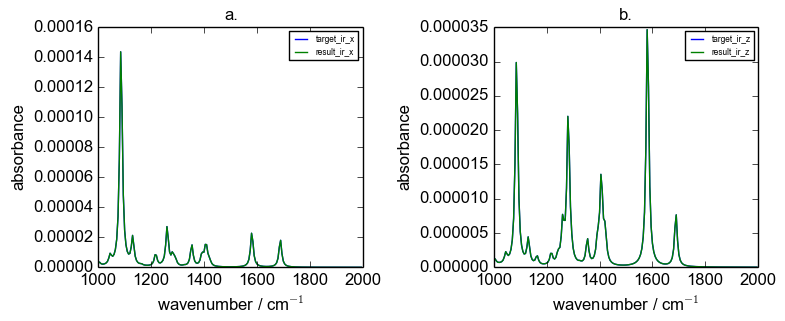
\includegraphics[scale=0.5]{Figures/chapter4_result_target_plotting_5datapoint_ir_version2.png}
\caption{IR spectra plotted by using target composition and return composition of Case 17. a. $x$-polarized IR spectra; b. $z$-polarized IR spectra.} \label{fig:4.2}
\end{figure}

\begin{figure}[!ht] 
\centering
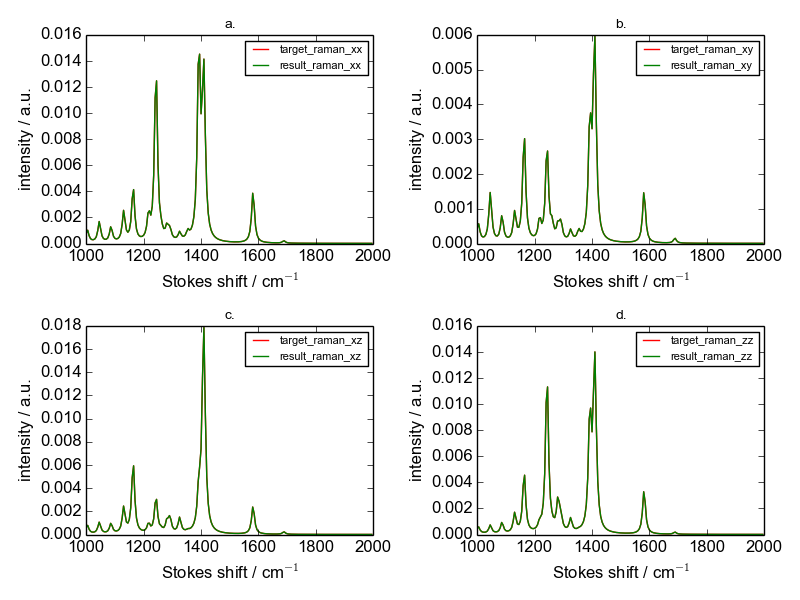
\includegraphics[scale=0.7]{Figures/chapter4_result_target_plotting_5datapoint_raman_version2.png}
\caption{Raman spectra plotted by using the target composition and the return composition of Case 17. a. $xx$-polarized Raman spectra; b. $xy$-polarized Raman spectra; c. $xz$-polarized Raman spectra; b. $zz$-polarized Raman spectra.} \label{fig:4.3}
\end{figure}

\begin{figure}[!ht]
\centering
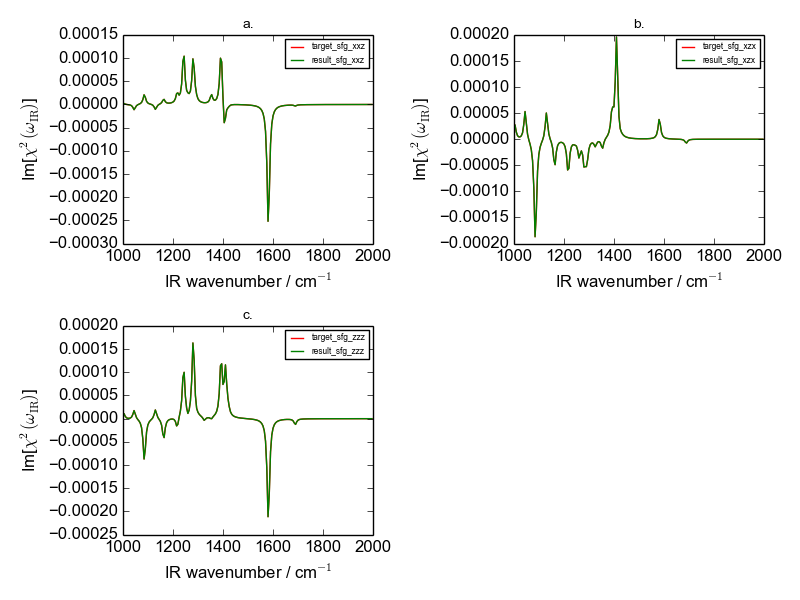
\includegraphics[scale=0.7]{Figures/chapter4_result_target_plotting_5datapoint_sfg_version2.png}
\caption{SFG spectra plotted by using the target composition and the return composition of Case 17. a. $xxz$-polarized SFG spectra; b. $xzx$-polarized SFG spectra; c. $zzz$-polarized SFG spectra.}  \label{fig:4.4}
\end{figure}

\begin{figure}[!ht] 
\centering
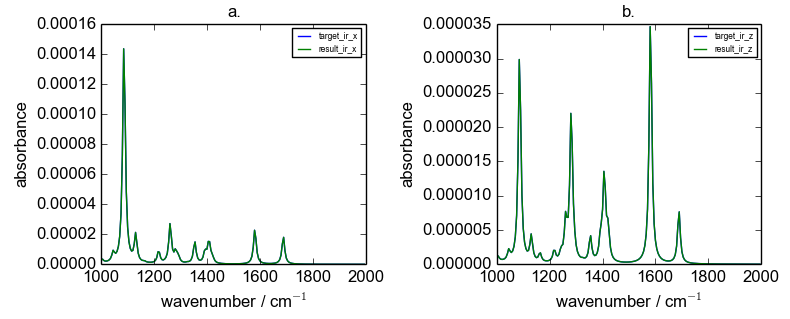
\includegraphics[scale=0.5]{Figures/chapter4_result_target_plotting_500datapoint_ir_version2.png}
\caption{IR spectra plotted by using the target composition and the return composition of Case 18. a. $x$-polarized IR spectra; b. $z$-polarized IR spectra.} \label{fig:4.5}
\end{figure}

\begin{figure}[!ht] 
\centering
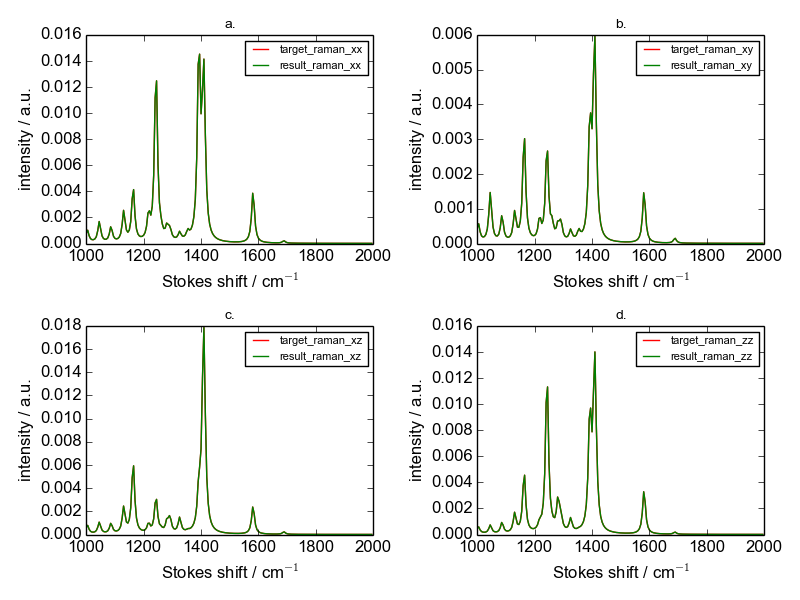
\includegraphics[scale=0.7]{Figures/chapter4_result_target_plotting_500datapoint_raman_version2.png}
\caption{Raman spectra plotted by using the target composition and the return composition of Case 18. a. $xx$-polarized Raman spectra; b. $xy$-polarized Raman spectra; c. $xz$-polarized Raman spectra; b. $zz$-polarized Raman spectra.} \label{fig:4.6}
\end{figure}

\begin{figure}[!ht] 
\centering
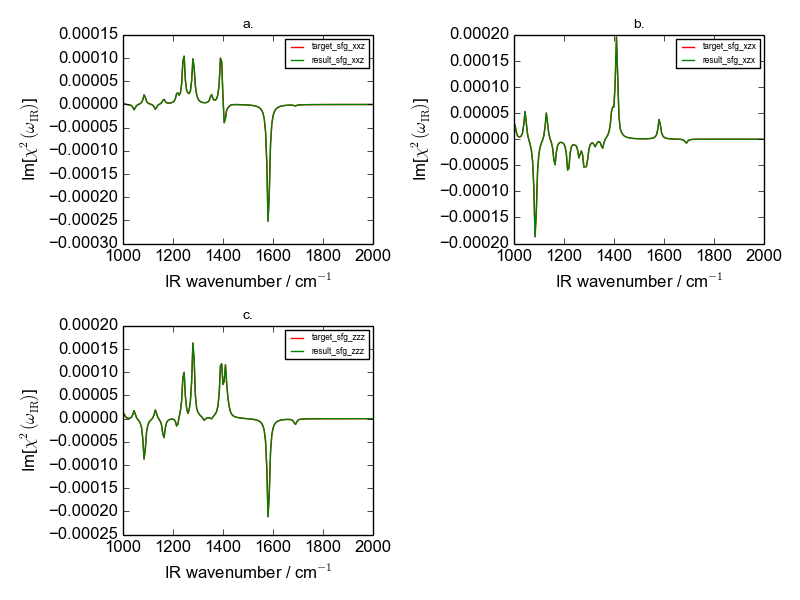
\includegraphics[scale=0.7]{Figures/chapter4_result_target_plotting_500datapoint_sfg_version2.png}
\caption{SFG spectra plotted by using the target composition and the return composition of Case 18. a. $xxz$-polarized SFG spectra; b. $xzx$-polarized SFG spectra; c. $zzz$-polarized SFG spectra.} \label{fig:4.7}
\end{figure} 

\section{Conclusion}



%\section{Extra Test Cases}
%TODO: this part of test cases are similar as what are done in Chapter 5 and 6. Think how to involve this part properly.

%From Case 1 to 18, LP model helps to return the target composition for some cases, and not for others. We want to figure out if there a clean line indicating the information used to generate the LP model is not sufficient to obtain the target composition for one molecule. In order to answer this question, more systematic test cases needed to be organized. Therefore, the following test cases are conducted. The Methionine candidate space is the same as Case 17 and 18. spread from $0^{\circ}$ to $80^{\circ}$ on $\theta$. 





